% -*- root: ../../main.tex -*- %

\subsection{Workflow and Activity Images} % (fold)
\label{sub:workflow_activity_images}
  To reap the benefits of the layer mechanism, the structure of the images should be chosen with care. Layers should be created in a way that enables reusability among the different use cases and they should be ordered by the frequency that they are changed with.

  The proposed structure of workflow and activity images, which is depicted in Figure~\ref{fig:layers_for_element_wrapping_containers} and reflected in the respective Dockerfiles \ref{fig:dockerfile_for_activity_base_image} and \ref{fig:dockerfile_for_workflow_base_image}, is thus as follows.

  The proposed structure consists on three images, which should build on each other consecutively, as they are meant to be increasingly specialized. The first image should provide the runtime environment. This image could be provided by a third-party vendor that specializes in building such images, \ie an \ac{OS} community or framework developers. Based on this image, a generic activity image \texttt{ac\_base} (and, for $*_{SEPC}^{*}$, a generic workflow image \texttt{wf\_base}) should be created. This image can be extended with element-specific information for each element of a workflow, when that workflow is exported for deployment, to yield the uppermost images \texttt{ac\_\$activity\_id} (and \texttt{wf\_\$workflow\_id}). An instance of this last image would then be a container with a suitable name of the form \texttt{aci\_\$activity\_instance\_id} (and respectively \texttt{wfi\_\$workflow\\\_instance\_id}).

  \begin{figure}[htbp]
    \centering
    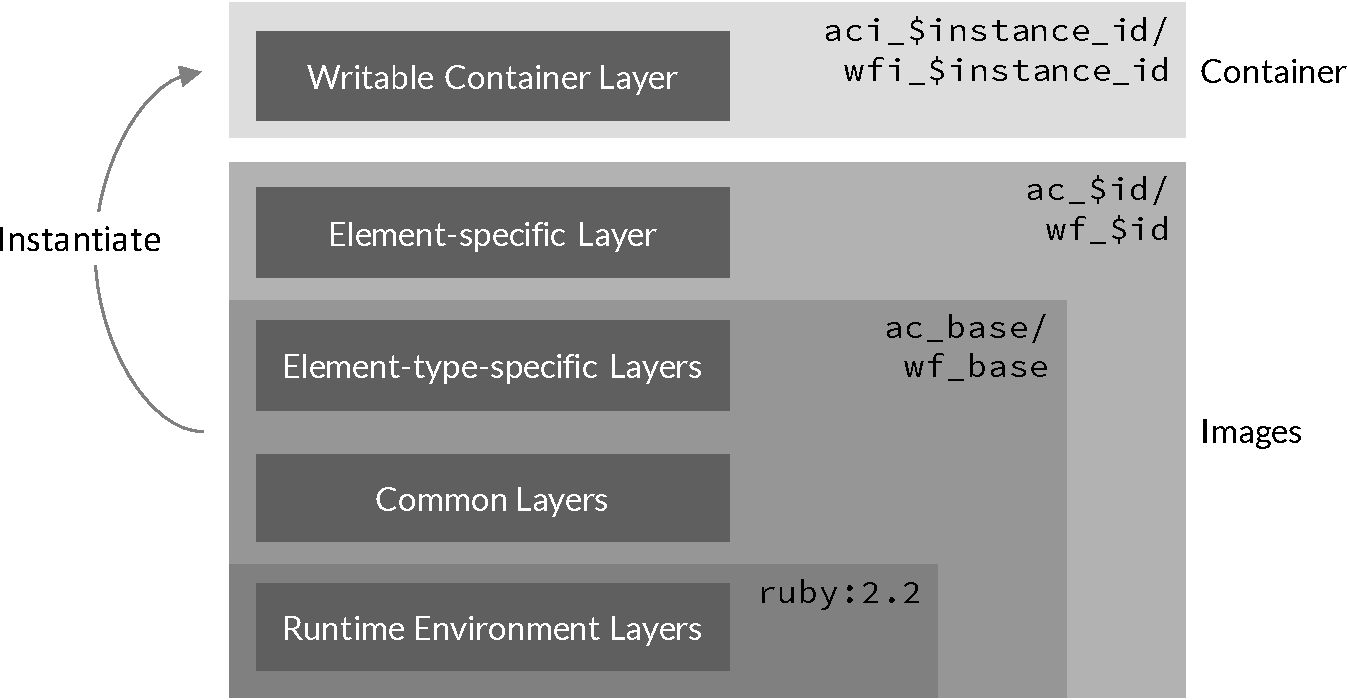
\includegraphics[width=0.95\textwidth]{content/images/layer_concept-crop.pdf}
    \caption{Layer Structure for Activity/Workflow Images}
    \label{fig:layers_for_element_wrapping_containers}
  \end{figure}

  Regarded in a more detailed fashion, the images' structure should look as follows.
  The foundation should be formed by \emph{runtime environment layers}, as they are expected to change rather seldom and are required by all derived images. Usually, these layers contain an \ac{OS}, common libraries and utility programs.

  The layers that form the \emph{$^*$\_base} images can be separated in two groups, \emph{common layers} and \emph{element-type-specific layers}. The \emph{element type} refers to either activity or workflow.
  The common layers should be created on top of these runtime environment layers. They are intended to contain the effects of invoked commands, added directory structures and files which are required by both activity images and workflow images. Even though no explicit name is given to these layers, they will be stored by Docker in its cache and used during the build process.

  In the next step, element-type-specific layers should be added. These layers are meant to contain data that is required for the execution of an activity \emph{or} a workflow, for example scripts which perform validation tasks (if they are not provided by a service) or general-purpose data transformation.

  The element-specific layer, which is added in the course of the export of an element (activity or workflow), contains files that are particular to single workflows or activities. In case of workflow images, for example, this layer would contain the process definition. In an activity image, it would contain the activity configuration and the schemata for data validation.

  By instantiating the resulting image a container is created at runtime, which owns the uppermost, writable layer. This is where the activity or workflow may store data that it needs during execution.

  At the time of writing, Docker registries do not yet reuse layers across repository borders during uploads, even though it is a proposed feature \cite{Mcgowan2015Proposal}. In order to benefit from the layering in the previously described way, it is thus necessary to let all activity images reside in the same repository by tagging them in the format

  \centerline{\texttt{\$repository\_url/activity}}

  and using the respective activity's \ac{ID} as a version tag to differentiate between them. They can then be referred to as

  \centerline{\texttt{\$repository\_url/activity:ac\_\$activity\_id}}

  Analogously, this is done with workflow images. Since it implies losing the internal image versioning mechanism, this solution should only be used as a workaround until cross-repository sharing of layers is possible.


\textcolor{red}{
  supported functions:
    - activity images
      - start subworkflow
      - start third-party container
      - initiate user input
    - workflow images
      - ggf wf engine
      - manage workdirectory (DV approaches)
}
% subsection workflow_activity_images (end)

\subsection{Communication} % (fold)
  \label{sub:application_level_communication}
  While the previous considerations were targeted at finding a model for the low-level communication, a way how the services communicate with each other

  - message queue between services
  - jeweilige protokolle via docker networks network between
  services publish/subscribe
% subsection application_level_communication (end)

  % \begin{sequencediagram}
    % \newinst{u}{Developer Gateway}
    % \newinst[1]{d}{Definition Service}
    % \newinst[1]{m}{MOM}
    % \newinst[1]{p}{Provisioner}

    % \mess{u}{subscribe}{m}
    % \mess{d}{subscribe}{m}
    % \mess{p}{subscribe}{m}

    % \mess{u}{wfms.wf.create}{m}
    % \mess{m}{wfms.wf.create}{d}
    % \mess{d}{wfms.wf.created}{m}
    % \mess{m}{wfms.wf.created}{u}
    % \mess{u}{wfms.pd.update}{m}
    % \mess{m}{wfms.pd.update}{d}
    % \mess{d}{wfms.pd.updated}{m}
    % \mess{m}{wfms.pd.updated}{u}
    % \mess{u}{wfms.wf.export}{m}
    % \mess{m}{wfms.wf.export}{d}
    % \mess{d}{wfms.wf.exported}{m}
    % \mess{m}{wfms.wf.exported}{p}
    % \mess{m}{wfms.wf.exported}{u}

  % \end{sequencediagram}

% subsection inter_component_communication (end)

\subsection{Components} % (fold)
  \label{sub:components}
  As noted in \ref{par:micro_services_architecture}, one of the downsides of \ac{MSA} is that it is crucial to determine suitable service boundaries. Some sources advise to first build a monolithic application and then analyze the result to single out services that can be extracted. In case of \acp{WfMS}, the identification of system components by the \ac{WFMC} for their reference model can be interpreted as such an analysis. Based on those components further micro-services for the prototype are then identified.

  As presented in \ref{sub:system_components}, the \ac{WFMC} identified the following components \cite[p.~13]{Hollingsworth1995Wfmc}:
    \begin{itemize}[nosep]
      \item Software Components
        \begin{itemize}[nosep]
          \item Definition Tool %
          \item Organization Modeling Tool %
          \item User Interface
          \item Workflow Engine(s)
          \item Worklists Handler %
        \end{itemize}
      \item Data Components
        \begin{itemize}[nosep]
          \item Organization Data %
          \item Process Definitions Data %
          \item Workflow Control Data
          \item Workflow Relevant Data %
          \item Worklists Data %
        \end{itemize}
    \end{itemize}

    ** draw communication diagram here **

  According to the \ac{WFMC}'s description, the definition tool, the worklists handler and the organization modeling tool each utilize a respective data component. Together with its respective datastore, each of them can be considered as an autonomous micro-service, since each would theoretically be able to provide its functionality without any further service.

  The workflow control data component can be considered as part of a workflow engine service.
  Depending on the chosen mode for the enactment, workflow relevant data is either managed by the workflow engine service, too, or accounted for by a data volume ($*_{*}^{DV}$). Only in the $*_{*}^{SER}$ variant, a dedicated service for its management and storage is needed.

  According to the decision to use the \ac{API} gateway pattern (\ref{sub:user_interaction_with_the_system}) to hide the internal system structure from its users, the two concact points -- one for administrative work and one for end-user work -- are realized using an appropriate gateway. The \emph{developer gateway} enables requests to the definition service, the infrastructure service and the organization management service through a \ac{GUI}. The \emph{user gateway} emits requests to the worklists service, wich are also issued through a \ac{GUI}.

  ** TODO: add deductions from objectives **
  In addition to the services derived above, the need for some additional services originates from considerations in \ref{sec:docker_for_wf_execution} and the objectives that were stated in \ref{sec:determination_of_objectives}.
  A Docker image registry was suggested to be used for the distribution of images to all nodes. Unless an external service such as Docker Hub is is used, an own registry service should be part of the \ac{WfMS}.
  The decision made in \ref{sub:application_level_communication} to use \ac{MOM} for the communication between services creates the need for a service which acts as such a middleware.
  To meet the requirement of automatically distributed images, a provisioning service should be introduced, which performs the appropriate actions. An infrastructure management service could be used to monitor the status and properties of the available nodes in the swarm.

  Besides the major components, independent functionalities which are frequently used could be singled out to separate services.
  %To demonstrate this exemplarily, a service which deals with the validation of input and output data is extracted for this prototype.
  One micro-service that might be extracted could for example address the validation of input and output data. Given a dataset and a set of rules on how to validate this dataset, such a service would be able to perform its task autonomously. As validation is a frequently recurring action in the execution of workflows -- before and after each activity and workflow -- it could thus be beneficial to be able to scale the execution of this task independently. **out of scope!**

  In the following, the resulting set of services is presented.

  \subsubsection{Workflow Definition Service} % (fold)
    \label{subs:workflow_definition_service}

    The workflow definition service encompasses the functions envisioned by the \ac{WFMC} as \emph{process definition tools}, \ie it is concerned with the analysis, modeling, description and documentation of business processes in form of workflow models and their process definitions. It further manages the assignment of activities to roles.

    With regards to its functional scope, the workflow definition service is also the service that should handle the transformation of workflows into their distributable format, \eg a self-contained description file or Docker images. In case of the latter, the workflow definition service would require access to a Docker daemon in order to perform the export. Once a workflow is transformed, the service should publish it. The transformations of workflows is performed by the \texttt{ImageBuilder} class, which relies on the \texttt{ProcessDefinitionImageSerializer} for the serialization of the process definition. The logic required for publishing the images is defined in the \texttt{ImageManager} class.

    The service should have \texttt{Workflow}, \texttt{Activity}, \texttt{ProcessDefinition}, and \texttt{ControlFlow} model classes, which provide the object-relational mapping for the respective objects. The roles assigned to activities have only to be dealt with in the form of unique identifiers, relying on the assumption that components which have to use them may resolve these identiefiers themselves.

    As a user interface is provided by the developer gateway service, the workflow definition service does not offer its own user interface, but rather exposes its functionality via the \ac{MOM}. This allows workflow definitions to be created and altered by arbitrary other services, \eg an conversion service which translates other process definition formats or some feedback mechanism that alters workflows based on their execution performance -- or a gateway service that provides an user interface.

    \begin{figure}[htbp]
      \centering
      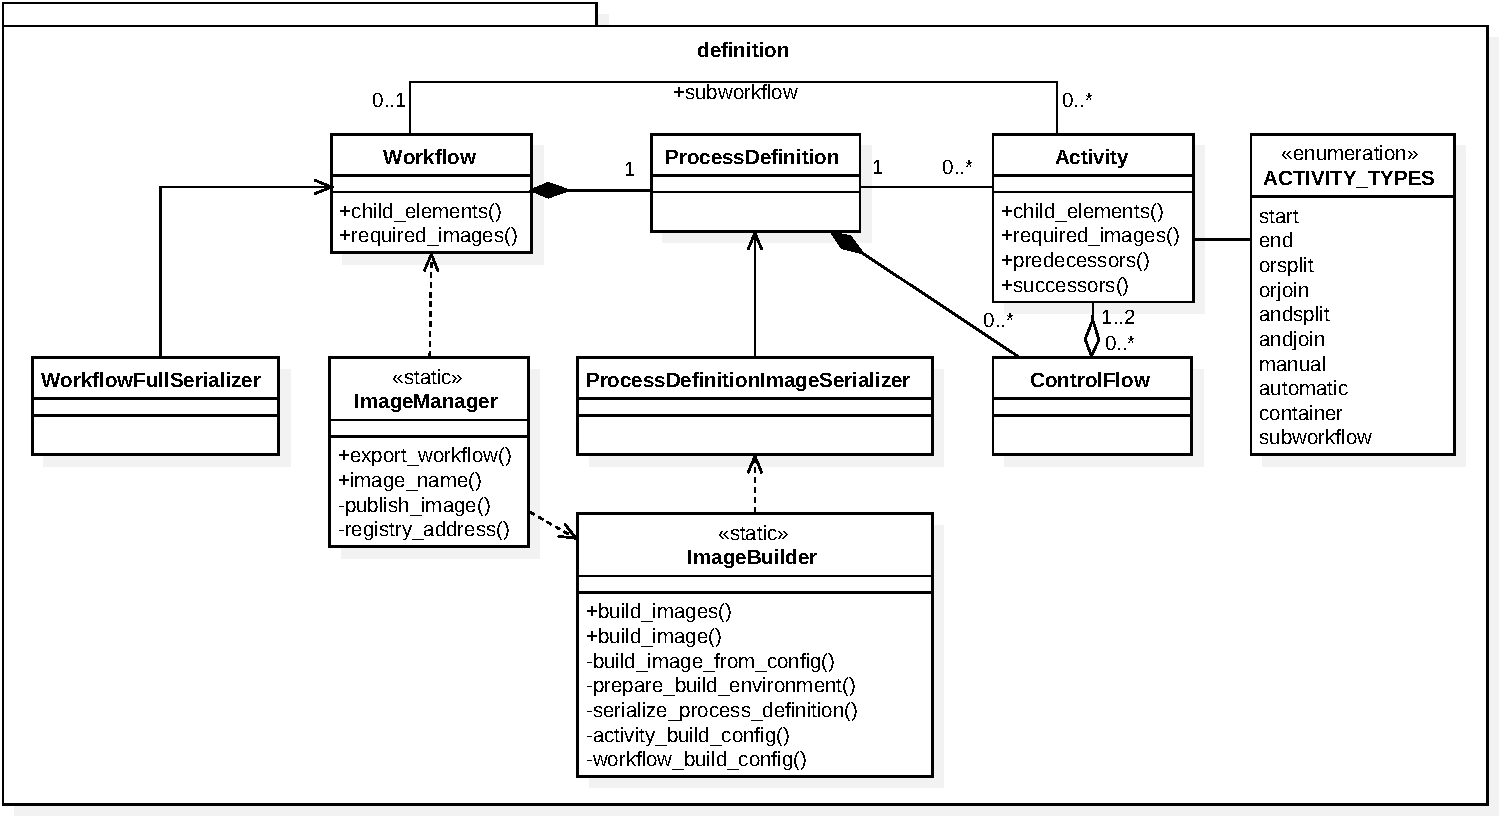
\includegraphics[width=0.95\textwidth]{content/images/class_diagram_definition-crop.pdf}
      \caption{UML Class Diagram for the Definition Service}
      \label{fig:uml_class_diagram_for_the_definition_service}
    \end{figure}

    In order react to requests of other services, the workflow definition service features consumer classes, which perform the required actions and publish a response, if required. \texttt{WorkflowConsumer}, \texttt{ActivityConsumer}, \texttt{ProcessDefinitionConsumer}, and \texttt{ControlFlowConsumer} response to \ac{CRUD} and index requests. The \texttt{WorkflowConsumer} additionally provides the means to react to requests for the export of a workflow.

    The serialization of a workflow with its components nested inside takes place in the \texttt{WorkflowFullSerializer}. Such a serialized version is required to avoid separte requests when the workflow is requested for modeling.

    Since one of the previously determined requirements for the prototype is that developers should be supported to use third-party images, the workflow definition service further reacts to relevant requests in the \texttt{DockerConsumer} by initiating a search for images with a specified name on Docker Hub.

    In order to be able to communicate with the \ac{MOM}, the workflow definition service is connected to the \texttt{wmfs\_backend} network.
    % ** As it is not actively involved in the enactment, it is not member of the \texttt{wfms\_enactment} network.
    % subsubsection workflow_definition_service (end)

  \subsubsection{Organization Management Service} % (fold)
    \label{subs:organization_management_service}
    The organization management service is part of the \emph{administration and monitoring tools}.
    As its name suggests, its functionality is aimed at the management of actors within an organization and their mutual relationships. The service may be queried for users or roles, or to authenticate users for the use of the \ac{WfMS}.

    The model classes \texttt{User} and \texttt{Role} provide the object-relational mapping for the database, while the \texttt{UserConsumer} and \texttt{RoleConsumer} classes enable the service to react to \ac{CRUD} and index requests that concern these objects.

    \begin{figure}[htbp]
      \centering
      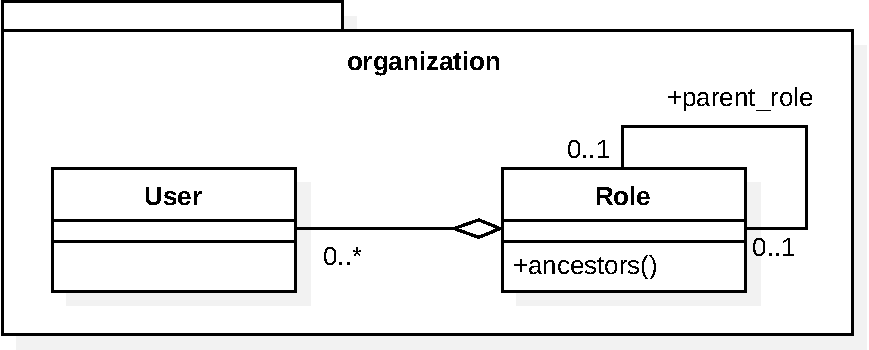
\includegraphics[width=0.65\textwidth]{content/images/class_diagram_organization-crop.pdf}
      \caption{UML Class Diagram for the Organization Service}
      \label{fig:uml_class_diagram_for_the_organization_service}
    \end{figure}

    Like the workflow definition service, the organization management service is connected to the \texttt{wmfs\_backend} network to be able to communicate with the \ac{MOM}.
    % subsubsection organization_management_service (end)

  \subsubsection{Worklist Service} % (fold)
    \label{subs:worklist_service}
    The sole responsibility of this service is the management of users' worklists. It should create, update and delete worklist items on request and publish the data submitted to it by users to the other services. If an user is deleted, it should remove the worklist item or reassign it to another user. The former tasks are performed by the \texttt{WorklistConsumer}, which reacts on related events. The latter task is in the responsibility of the \texttt{UserConsumer}, which reacts to the deletion of an user. The worklist item's object-relational mapping is performed by the \texttt{WorklistItem} model class.
    % subsubsection worklist_service (end)

  \subsubsection{Workflow Engine Service} % (fold)
    \label{subs:workflow_engine_service}
    ** TODO: incomplete **
    In wide parts, the workflow engine service is congruent to the \emph{workflow engine} component identified by the \ac{WFMC} in terms of functionality, which is described in \ref{par:workflow_engine}. The way  to utilize Docker for the workflow enactment chosen in \ref{sec:docker_for_wf_execution} has an impact on the range of functionalities that this service has, though.

    - choose participants
    - add to execution networks

    WorkflowConsumer
    WorkflowInstanceConsumer
    ServerConsumer
    WorkflowInstance
    WorkflowScheduler


    The extent to which the workflow engine service controls the instanciation of workflow components depends on .
    % subsubsection workflow_engine_service (end)

  \subsubsection{Developer Gateway} % (fold)
    \label{subs:developer_gateway}
    Since it only offers a unified access to the \ac{WfMS} and does not store any data itself, the developer gateway does not require any database. The service is realized in a two-tier architecture, with a backend part that handles requests to and responses from the various \ac{WfMS} services, and a frontend part that presents the reeived data to the developers and accepts their input.

    The only task of the backend is forwarding the user's requests to the message queue and the corresponding responses back to the user. The controller classes that are responsible for this (\texttt{ActivitesController}, \texttt{ControlFlowsController}, \texttt{DockerController}, \texttt{ProcessDefinitionsController}, \texttt{RolesController}, \texttt{ServersController}, \texttt{UsersController}, \texttt{WorkflowsController}) are thus very lean -- they only contain the logic to forward requests to suitable routing keys. Each of them inherits from the \texttt{ApplicationController}, which manages the messaging logic and gives access to a shared single connection to the \ac{MOM}.

    The \texttt{TemplatesController} is different from the other controller classes, as is not involved in forwarding requests, but serves the only purpose to render and deliver the \ac{HTML} fragments required by the frontend.

    This service and the user gateway service are intended to be the only services that can be reached from outside of the \ac{WfMS}.

    % ** - provides access to
    %   - infrastructure
    %   - definition
    %   - organization
    % - gives a visual modeling interface for workflows
    % subsubsection developer_gateway (end)

  \subsubsection{User Gateway} % (fold)
    \label{subs:user_gateway}
    Analogous to the developer gateway, the user gateway provides access to those \ac{WfMS} services that are relevant to its users, that is, in the chosen setup, only the worklist management service.

    Due to the few responsibilities of this gateway, there exist only two controller classes: \texttt{WorklistItemsController}, which forwards \ac{CRUD} requests that concern worklist items and \texttt{WorklistController}, which provides the means to obtain all existing worklists.
    % subsubsection user_gateway (end)


  % \subsubsection{Validation Service} % (fold)
    %   \label{subs:valitation_service}
    %   One micro-service that might be extracted from the above services concerns the validation of data. Given a dataset and a set of rules on how to validate this dataset, the service is able to perform its task autonomously. As validation is a frequently recurring action in the execution of workflows -- before and after each activity and workflow -- it could thus be beneficial to be able to scale the execution of this task independently.
    %   % subsubsection valitation_service (end)

  \subsubsection{Infrastructure Management Service} % (fold)
    \label{subs:environment_management_service}
    The infrastructure management service fetches and refines the information related to the swarms nodes.
    That is, it lists all nodes and can return their properties, (running) containers and available images.
    Supported by the \texttt{DockerHelper}, which provides the connections to the different nodes, the \texttt{EnvironmentManager} contains the required logic to fulfil thise tasks. The \texttt{ServerConsumer} waits for relevant requests via the \ac{MOM}, instructs the \texttt{EnvironmentManager} accordingly, and returns the results. Further, there is a \texttt{Server} model class, which is used to structure the obtained information.

    Additionally to its role in the information retrieval, the \texttt{EnvironmentManager} listens for  new nodes in the swarm and launches the provisioning service on joining nodes.
    % subsubsection environment_management_service (end)

  \subsubsection{Registry} % (fold)
  \label{subs:registry}
    All solutions presented in Section~\ref{sec:docker_for_wf_execution} feature custom Docker images, be it workers or contanierized activities or workflows. These images presumably contain information on business processes and other information whose disclosure should be avoided.  In order to store and distribute these images, a private registry is thus required. A possible alternative for less sensitive images could be the utilization of a private remote repository on the Docker Hub.
  % subsubsection registry (end)

  \subsubsection{Provisioning Service} % (fold)
    \label{subs:provisioning_service}
    The objectives include the reduction of administrative work. In order to prevent the user from having to distribute the Docker images required for the execution of workflows manually, a service should perform this task. This service should provision each machine with said images whenever such an image is created or updated. To do so, the \texttt{ImageConsumer} and \texttt{ServerConsumer} classes react to relevant events by invoking the appropriate Docker commands.

    The service could either run as an instance on each machine, performing the required Docker operations locally, or run on the Docker Swarm master machine as one instance and perform the operations remotely on all machines.

    **perform what, when?**
    % subsubsection provisioning_service (end)
% subsection components (end)

